\documentclass[11pt]{article}
% switch to [review] for anonymous submission
\usepackage[final]{acl}
\usepackage{times}
\usepackage{latexsym}
\usepackage[T1]{fontenc}
\usepackage[utf8]{inputenc}
\usepackage{microtype}
\usepackage{inconsolata}
\usepackage{graphicx}
\usepackage{booktabs}
\usepackage{amsmath,amssymb}

\newcommand{\rhot}{\rho_{\text{tr}}}
\newcommand{\dec}{\textsc{Dec}}
\newcommand{\cfn}{\textsc{CF}_{N}}
\newcommand{\cft}{\textsc{CF}_{T}}
\newcommand{\conf}{\textsc{Conflict}}
\newcommand{\leak}{\textsc{Leak}}
\newcommand{\absCFbiosGFive}{.03}
\newcommand{\absCFbiosGNine}{.15}
\newcommand{\absCFbiosQFive}{.03}
\newcommand{\absCFbiosQNine}{.17}
\newcommand{\absCFcebabGFive}{.23}
\newcommand{\absCFcebabGNine}{.44}
\newcommand{\absCFcebabQFive}{.25}
\newcommand{\absCFcebabQNine}{.60}
\newcommand{\absCFcivilGFive}{.08}
\newcommand{\absCFcivilGNine}{.31}
\newcommand{\absCFcivilQFive}{.09}
\newcommand{\absCFcivilQNine}{.36}
\newcommand{\cfNnbMax}{.89}
\newcommand{\cfNnbMin}{$-$.10}
\newcommand{\cfTmax}{1.19}
\newcommand{\cfTmin}{.84}
\newcommand{\corrCFmax}{+.39}
\newcommand{\corrCFmin}{$-$.61}
\newcommand{\corrCFnNS}{3}
\newcommand{\corrCFnSigNeg}{2}
\newcommand{\corrCFnSigPos}{1}
\newcommand{\cosMaxbios}{.18}
\newcommand{\cosMaxcebab}{.83}
\newcommand{\cosMaxcivil}{.17}
\newcommand{\cosMinbios}{.06}
\newcommand{\cosMincebab}{.66}
\newcommand{\cosMincivil}{$-$.39}
\newcommand{\eqCFmaxbiosGFive}{.03}
\newcommand{\eqCFmaxbiosGNine}{.29}
\newcommand{\eqCFmaxbiosQFive}{.05}
\newcommand{\eqCFmaxbiosQNine}{.41}
\newcommand{\eqCFmaxcebabGFive}{.02}
\newcommand{\eqCFmaxcebabGNine}{.63}
\newcommand{\eqCFmaxcebabQFive}{.09}
\newcommand{\eqCFmaxcebabQNine}{.81}
\newcommand{\eqCFmaxcivilGFive}{$-$.02}
\newcommand{\eqCFmaxcivilGNine}{.35}
\newcommand{\eqCFmaxcivilQFive}{.03}
\newcommand{\eqCFmaxcivilQNine}{.37}
\newcommand{\eqCFminbiosGFive}{$-$.06}
\newcommand{\eqCFminbiosGNine}{.09}
\newcommand{\eqCFminbiosQFive}{$-$.03}
\newcommand{\eqCFminbiosQNine}{.08}
\newcommand{\eqCFmincebabGFive}{.01}
\newcommand{\eqCFmincebabGNine}{.25}
\newcommand{\eqCFmincebabQFive}{.09}
\newcommand{\eqCFmincebabQNine}{.54}
\newcommand{\eqCFmincivilGFive}{$-$.03}
\newcommand{\eqCFmincivilGNine}{.35}
\newcommand{\eqCFmincivilQFive}{$-$.00}
\newcommand{\eqCFmincivilQNine}{.28}
\newcommand{\eqNbiosGFive}{55}
\newcommand{\eqNbiosGNine}{63}
\newcommand{\eqNbiosQFive}{54}
\newcommand{\eqNbiosQNine}{66}
\newcommand{\eqNcebabGFive}{2}
\newcommand{\eqNcebabGNine}{8}
\newcommand{\eqNcebabQFive}{1}
\newcommand{\eqNcebabQNine}{9}
\newcommand{\eqNcivilGFive}{2}
\newcommand{\eqNcivilGNine}{1}
\newcommand{\eqNcivilQFive}{2}
\newcommand{\eqNcivilQNine}{4}
\newcommand{\fpCFlrbiosGFive}{$-$.01}
\newcommand{\fpCFlrbiosGNine}{.20}
\newcommand{\fpCFlrbiosQFive}{$-$.00}
\newcommand{\fpCFlrbiosQNine}{.20}
\newcommand{\fpCFlrcebabGFive}{$-$.00}
\newcommand{\fpCFlrcebabGNine}{.63}
\newcommand{\fpCFlrcebabQFive}{.13}
\newcommand{\fpCFlrcebabQNine}{.83}
\newcommand{\fpCFlrcivilGFive}{.01}
\newcommand{\fpCFlrcivilGNine}{.26}
\newcommand{\fpCFlrcivilQFive}{.06}
\newcommand{\fpCFlrcivilQNine}{.40}
\newcommand{\fpCFnebiosGFive}{$-$.03}
\newcommand{\fpCFnebiosGNine}{.06}
\newcommand{\fpCFnebiosQFive}{$-$.02}
\newcommand{\fpCFnebiosQNine}{.06}
\newcommand{\fpCFnecebabGFive}{$-$.01}
\newcommand{\fpCFnecebabGNine}{.14}
\newcommand{\fpCFnecebabQFive}{.02}
\newcommand{\fpCFnecebabQNine}{.34}
\newcommand{\fpCFnecivilGFive}{$-$.01}
\newcommand{\fpCFnecivilGNine}{.18}
\newcommand{\fpCFnecivilQFive}{.04}
\newcommand{\fpCFnecivilQNine}{.28}
\newcommand{\fpDdbiosGFive}{$-$.000}
\newcommand{\fpDdbiosGNine}{+.001}
\newcommand{\fpDdbiosQFive}{+.000}
\newcommand{\fpDdbiosQNine}{+.001}
\newcommand{\fpDdcebabGFive}{+.000}
\newcommand{\fpDdcebabGNine}{+.004}
\newcommand{\fpDdcebabQFive}{$-$.003}
\newcommand{\fpDdcebabQNine}{+.009}
\newcommand{\fpDdcivilGFive}{+.008}
\newcommand{\fpDdcivilGNine}{+.039}
\newcommand{\fpDdcivilQFive}{+.011}
\newcommand{\fpDdcivilQNine}{+.049}
\newcommand{\fpEqbiosGFive}{yes}
\newcommand{\fpEqbiosGNine}{yes}
\newcommand{\fpEqbiosQFive}{yes}
\newcommand{\fpEqbiosQNine}{yes}
\newcommand{\fpEqcebabGFive}{yes}
\newcommand{\fpEqcebabGNine}{no}
\newcommand{\fpEqcebabQFive}{yes}
\newcommand{\fpEqcebabQNine}{no}
\newcommand{\fpEqcivilGFive}{no}
\newcommand{\fpEqcivilGNine}{no}
\newcommand{\fpEqcivilQFive}{no}
\newcommand{\fpEqcivilQNine}{no}
\newcommand{\fpHibiosGFive}{+.000}
\newcommand{\fpHibiosGNine}{+.002}
\newcommand{\fpHibiosQFive}{+.000}
\newcommand{\fpHibiosQNine}{+.002}
\newcommand{\fpHicebabGFive}{+.001}
\newcommand{\fpHicebabGNine}{+.012}
\newcommand{\fpHicebabQFive}{+.000}
\newcommand{\fpHicebabQNine}{+.023}
\newcommand{\fpHicivilGFive}{+.011}
\newcommand{\fpHicivilGNine}{+.049}
\newcommand{\fpHicivilQFive}{+.015}
\newcommand{\fpHicivilQNine}{+.062}
\newcommand{\fpLobiosGFive}{$-$.000}
\newcommand{\fpLobiosGNine}{$-$.001}
\newcommand{\fpLobiosQFive}{$-$.000}
\newcommand{\fpLobiosQNine}{+.000}
\newcommand{\fpLocebabGFive}{$-$.000}
\newcommand{\fpLocebabGNine}{$-$.003}
\newcommand{\fpLocebabQFive}{$-$.006}
\newcommand{\fpLocebabQNine}{$-$.003}
\newcommand{\fpLocivilGFive}{+.005}
\newcommand{\fpLocivilGNine}{+.031}
\newcommand{\fpLocivilQFive}{+.006}
\newcommand{\fpLocivilQNine}{+.036}
\newcommand{\geomMAEbios}{.02}
\newcommand{\geomMAEcebab}{.12}
\newcommand{\geomPearsonbios}{.33}
\newcommand{\geomPearsoncebab}{.43}
\newcommand{\gptPlaceboAccMax}{.98}
\newcommand{\gptPlaceboAccMin}{.92}
\newcommand{\kappaMax}{.42}
\newcommand{\kappaMin}{.05}
\newcommand{\nbBestbiosGFive}{.995}
\newcommand{\nbBestbiosGNine}{.998}
\newcommand{\nbBestbiosGSeven}{.995}
\newcommand{\nbBestbiosQFive}{.995}
\newcommand{\nbBestbiosQNine}{.998}
\newcommand{\nbBestbiosQSeven}{.995}
\newcommand{\nbBestcebabGFive}{.960}
\newcommand{\nbBestcebabGNine}{.979}
\newcommand{\nbBestcebabGSeven}{.967}
\newcommand{\nbBestcebabQFive}{.924}
\newcommand{\nbBestcebabQNine}{.966}
\newcommand{\nbBestcebabQSeven}{.934}
\newcommand{\nbBestcivilGFive}{.839}
\newcommand{\nbBestcivilGNine}{.940}
\newcommand{\nbBestcivilGSeven}{.869}
\newcommand{\nbBestcivilQFive}{.829}
\newcommand{\nbBestcivilQNine}{.932}
\newcommand{\nbBestcivilQSeven}{.859}
\newcommand{\nbCFmaxbiosGFive}{.03}
\newcommand{\nbCFmaxbiosGNine}{.29}
\newcommand{\nbCFmaxbiosGSeven}{.10}
\newcommand{\nbCFmaxbiosQFive}{.04}
\newcommand{\nbCFmaxbiosQNine}{.41}
\newcommand{\nbCFmaxbiosQSeven}{.13}
\newcommand{\nbCFmaxcebabGFive}{.08}
\newcommand{\nbCFmaxcebabGNine}{.72}
\newcommand{\nbCFmaxcebabGSeven}{.26}
\newcommand{\nbCFmaxcebabQFive}{.28}
\newcommand{\nbCFmaxcebabQNine}{.89}
\newcommand{\nbCFmaxcebabQSeven}{.54}
\newcommand{\nbCFmaxcivilGFive}{.07}
\newcommand{\nbCFmaxcivilGNine}{.50}
\newcommand{\nbCFmaxcivilGSeven}{.19}
\newcommand{\nbCFmaxcivilQFive}{.08}
\newcommand{\nbCFmaxcivilQNine}{.45}
\newcommand{\nbCFmaxcivilQSeven}{.17}
\newcommand{\nbCFminbiosGFive}{$-$.07}
\newcommand{\nbCFminbiosGNine}{.08}
\newcommand{\nbCFminbiosGSeven}{$-$.01}
\newcommand{\nbCFminbiosQFive}{$-$.04}
\newcommand{\nbCFminbiosQNine}{.08}
\newcommand{\nbCFminbiosQSeven}{.00}
\newcommand{\nbCFmincebabGFive}{$-$.10}
\newcommand{\nbCFmincebabGNine}{.26}
\newcommand{\nbCFmincebabGSeven}{.05}
\newcommand{\nbCFmincebabQFive}{.02}
\newcommand{\nbCFmincebabQNine}{.46}
\newcommand{\nbCFmincebabQSeven}{.15}
\newcommand{\nbCFmincivilGFive}{$-$.02}
\newcommand{\nbCFmincivilGNine}{.30}
\newcommand{\nbCFmincivilGSeven}{.09}
\newcommand{\nbCFmincivilQFive}{.04}
\newcommand{\nbCFmincivilQNine}{.24}
\newcommand{\nbCFmincivilQSeven}{.14}
\newcommand{\nbConfMaxbiosGFive}{.99}
\newcommand{\nbConfMaxbiosGNine}{.97}
\newcommand{\nbConfMaxbiosGSeven}{.99}
\newcommand{\nbConfMaxbiosQFive}{.99}
\newcommand{\nbConfMaxbiosQNine}{.97}
\newcommand{\nbConfMaxbiosQSeven}{.99}
\newcommand{\nbConfMaxcebabGFive}{.95}
\newcommand{\nbConfMaxcebabGNine}{.82}
\newcommand{\nbConfMaxcebabGSeven}{.93}
\newcommand{\nbConfMaxcebabQFive}{.90}
\newcommand{\nbConfMaxcebabQNine}{.69}
\newcommand{\nbConfMaxcebabQSeven}{.86}
\newcommand{\nbConfMaxcivilGFive}{.84}
\newcommand{\nbConfMaxcivilGNine}{.43}
\newcommand{\nbConfMaxcivilGSeven}{.69}
\newcommand{\nbConfMaxcivilQFive}{.83}
\newcommand{\nbConfMaxcivilQNine}{.41}
\newcommand{\nbConfMaxcivilQSeven}{.71}
\newcommand{\nbConfMinbiosGFive}{.98}
\newcommand{\nbConfMinbiosGNine}{.92}
\newcommand{\nbConfMinbiosGSeven}{.96}
\newcommand{\nbConfMinbiosQFive}{.98}
\newcommand{\nbConfMinbiosQNine}{.83}
\newcommand{\nbConfMinbiosQSeven}{.96}
\newcommand{\nbConfMincebabGFive}{.93}
\newcommand{\nbConfMincebabGNine}{.57}
\newcommand{\nbConfMincebabGSeven}{.86}
\newcommand{\nbConfMincebabQFive}{.84}
\newcommand{\nbConfMincebabQNine}{.44}
\newcommand{\nbConfMincebabQSeven}{.70}
\newcommand{\nbConfMincivilGFive}{.83}
\newcommand{\nbConfMincivilGNine}{.29}
\newcommand{\nbConfMincivilGSeven}{.66}
\newcommand{\nbConfMincivilQFive}{.81}
\newcommand{\nbConfMincivilQNine}{.35}
\newcommand{\nbConfMincivilQSeven}{.64}
\newcommand{\nbNbiosGFive}{60}
\newcommand{\nbNbiosGNine}{66}
\newcommand{\nbNbiosGSeven}{61}
\newcommand{\nbNbiosQFive}{58}
\newcommand{\nbNbiosQNine}{66}
\newcommand{\nbNbiosQSeven}{62}
\newcommand{\nbNcebabGFive}{11}
\newcommand{\nbNcebabGNine}{39}
\newcommand{\nbNcebabGSeven}{13}
\newcommand{\nbNcebabQFive}{10}
\newcommand{\nbNcebabQNine}{37}
\newcommand{\nbNcebabQSeven}{18}
\newcommand{\nbNcivilGFive}{5}
\newcommand{\nbNcivilGNine}{12}
\newcommand{\nbNcivilGSeven}{9}
\newcommand{\nbNcivilQFive}{4}
\newcommand{\nbNcivilQNine}{8}
\newcommand{\nbNcivilQSeven}{5}
\newcommand{\neShareMinLeak}{67\%}
\newcommand{\nuisAbsNineMax}{.60}
\newcommand{\nuisAbsNineMin}{.15}
\newcommand{\obsMaxbios}{.04}
\newcommand{\obsMaxcebab}{.85}
\newcommand{\obsMaxcivil}{.13}
\newcommand{\obsMinbios}{.02}
\newcommand{\obsMincebab}{.63}
\newcommand{\obsMincivil}{.04}
\newcommand{\placeboMax}{.07}
\newcommand{\placeboMin}{.01}
\newcommand{\placebobiosGFive}{.01}
\newcommand{\placebobiosGNine}{.01}
\newcommand{\placebobiosQFive}{.02}
\newcommand{\placebobiosQNine}{.02}
\newcommand{\placebocebabGFive}{.04}
\newcommand{\placebocebabGNine}{.04}
\newcommand{\placebocebabQFive}{.06}
\newcommand{\placebocebabQNine}{.06}
\newcommand{\placebocivilGFive}{.05}
\newcommand{\placebocivilGNine}{.05}
\newcommand{\placebocivilQFive}{.05}
\newcommand{\placebocivilQNine}{.07}
\newcommand{\predMaxbios}{.07}
\newcommand{\predMaxcebab}{.92}
\newcommand{\predMaxcivil}{.25}
\newcommand{\predMinbios}{.03}
\newcommand{\predMincebab}{.76}
\newcommand{\predMincivil}{$-$.74}
\newcommand{\qwenPlaceboAccMax}{.60}
\newcommand{\qwenPlaceboAccMin}{.44}
\newcommand{\robAbsMinSevenUp}{.89}
\newcommand{\robAllValMin}{.77}
\newcommand{\robSDMin}{.87}
\newcommand{\selFullConfCFmax}{.34}
\newcommand{\selFullConfCFmin}{.17}
\newcommand{\selFullConfDecMeanWorst}{.036}
\newcommand{\selFullConfDecWorst}{.049}
\newcommand{\selNcells}{36}
\newcommand{\selNfailCells}{3}
\newcommand{\selStdConfAllSeeds}{True}
\newcommand{\selStdConfCFmax}{.15}
\newcommand{\selStdConfCFmin}{.08}
\newcommand{\selStdConfDecMeanWorst}{.018}
\newcommand{\selStdConfDecWorst}{.023}
\newcommand{\sgnCFbiosGFive}{$-$.03}
\newcommand{\sgnCFbiosGNine}{.15}
\newcommand{\sgnCFbiosQFive}{$-$.02}
\newcommand{\sgnCFbiosQNine}{.17}
\newcommand{\sgnCFcebabGFive}{$-$.02}
\newcommand{\sgnCFcebabGNine}{.41}
\newcommand{\sgnCFcebabQFive}{.07}
\newcommand{\sgnCFcebabQNine}{.59}
\newcommand{\sgnCFcivilGFive}{.02}
\newcommand{\sgnCFcivilGNine}{.30}
\newcommand{\sgnCFcivilQFive}{.04}
\newcommand{\sgnCFcivilQNine}{.35}
\newcommand{\synCFRangeStdMax}{.87}
\newcommand{\synCFRangeStdMin}{.83}
\newcommand{\synDecRangeNe}{.09}
\newcommand{\synDecRangeStd}{.03}


\title{Decodability Is Not Validity: Evaluating Nuisance Sensitivity\\in Language Model Concept Probes}

\author{Ayal Klein \\
  \texttt{ayalk@ariel.ac.il}}

\begin{document}
\maketitle

\begin{abstract}
Two concept probes can be equally accurate at predicting a concept from a language model's hidden states while their scores contain different mixtures of the target concept and a correlated nuisance attribute. We measure how often this happens and what it costs. Across three public datasets that pair a target with a different kind of nuisance (two aspect sentiments; occupation and gender; toxicity and identity mention), two LLMs, and a population of concept extractors, we compare decodability with discriminant evidence about one named nuisance: the score's dependence on the nuisance with the target held fixed, and its response to input edits intended to change only the nuisance, filtered by two LLM judges and compared against placebo edits. Under correlated training data, extractors that are statistically equivalent in held-out AUROC differ several-fold in nuisance sensitivity; decodability is not a reliable proxy for it, and its relationship to nuisance sensitivity changes sign across settings. Where target edits exist (CEBaB), competitive extractors pass them regardless of nuisance sensitivity. Selecting extractors with nuisance-aware development diagnostics, which need nuisance labels but no counterfactuals, lowers counterfactual nuisance sensitivity at a modest accuracy cost. Concept measurements should be validated, not just decoded.
\end{abstract}

\section{Introduction}

Probes, concept activation vectors and subspace readouts turn a hidden state into a scalar proxy for a concept $T$ in the input \citep{alain2017understanding,kim2018tcav,belinkov2022probing,zou2023representation,marks2024geometry}; the usual evidence for that reading is decodability, i.e.\ predicting held-out labels of $T$. Decodability cannot identify \emph{what} the score measures. For binary $T$ and a nuisance $N$, the scores $s_1=T$ and $s_2=T+\alpha N$ with $0<\alpha<1$ both rank $T$ perfectly, yet only $s_2$ moves when $N$ alone changes. When two extractors are equally accurate, nothing in their accuracy says which one is more selective for $T$.

Measurement theory treats this as a question of construct validity, an evidential and multidimensional property of a score's interpretation rather than a number the score has \citep{cronbach1955construct,messick1995validity,jacobs2021measurement,bean2025measuring}. Part of that evidence is \emph{discriminant}: the score should reflect the intended construct rather than a distinct, possibly correlated one \citep{campbell1959convergent}. Valid measures of correlated constructs can correlate; what discriminant evidence asks is whether the score depends on the other construct \emph{once the target is held fixed}. We study exactly this, for one named nuisance per dataset; passing our tests is necessary evidence about that nuisance, not evidence of validity in general.

That accuracy cannot detect such dependence is not new: probes trained on spuriously correlated data can rely on the spurious attribute \citep{kumar2022probing}, probing accuracy need not reflect use by the model \citep{hewitt2019designing,ravichander2021probing,elazar2021amnesic}, and interventions on representations trade completeness against selectivity \citep{canby2025reliable,huang2024ravel}. Recent work tests whether probes and SAEs disentangle known concepts \citep{mueller2026isolation}, compares concept-subspace estimators \citep{naowarat2026framework}, shows accurate probes can be misaligned \citep{lysnaeslarsen2025probing}, and links embedding-based social measures to confounding and counterfactual validation \citep{li2026proxy}. We ask a narrower question about scalar readouts: among extractors that are accuracy-matched on held-out data, how much does sensitivity to a named nuisance under input edits vary, does it persist without training-set correlation, and can development diagnostics choose better? We answer with a population study over three variable types and two models, using judge-filtered, placebo-controlled input edits (\S\ref{sec:results}), and a comparison of development-set selection criteria (\S\ref{sec:selection}). Our interventions edit the \emph{input text} of frozen models; we make no claim that the extracted directions causally mediate model behavior.

\section{Measuring nuisance selectivity}
\label{sec:battery}

An \emph{extractor} maps a hidden state $h$ to $s(h)=w^\top z(h)+b$, with $z$ the standardization on training data; subspace methods have a linear readout too, so every extractor is a scalar score. Each dataset supplies a binary target $T$, a binary nuisance $N$ correlated with $T$ in natural data, and edits of the input. Let \mbox{$\rho=P(N{=}1\mid T{=}1)$} \mbox{${}=P(N{=}0\mid T{=}0)$} with balanced $T$. Extractors are trained at $\rhot\in\{0.5,0.7,0.9\}$; test metrics reweight the four $(T,N)$ cells of one fixed test pool.

\noindent\textbf{\dec{}}: AUROC of $s$ for $T$ at $\rho=\rhot$ (in-distribution decodability, the standard criterion).\\
\textbf{$|$\leak{}$|$}: $\tfrac12\sum_{t}|\mathrm{AUROC}(s\to N\mid T{=}t)-0.5|$, dependence on $N$ with the target held fixed. The absolute form avoids cancelling opposite dependences in the two target classes.\\
\textbf{\conf{}}: AUROC for $T$ on the cells with $T\neq N$ (a fully reversed correlation). A stress test, not a validity measure: there, $s=-N$ also ranks $T$ perfectly.\\
\textbf{$\cfn$}: mean change in $s$ under edits that flip only $N$, signed toward the $N$ value that co-occurs with $T{=}1$, divided by the mean score gap between the $T$ classes on the decorrelated pool ($\Delta_T$). As a signed mean can hide opposite changes, we also report $|\cfn|$ (mean absolute change over $\Delta_T$) and compare with \emph{placebo} edits that change neither variable.\\
\textbf{$\cft$}: the same quantity for edits that flip $T$ (CEBaB only), i.e.\ convergent counterfactual evidence.

\section{Setup}
\label{sec:setup}

\begin{table}[t]
\centering\small\setlength{\tabcolsep}{2pt}
\resizebox{\columnwidth}{!}{\begin{tabular}{@{}llccc@{}}
\toprule
 & target $T$ / nuisance $N$ & $N$ edits & judged by both & accepted \\
\midrule
CEBaB & service / food sentiment & 210 & 210 & 41\% \\
BiasBios & surgeon vs.\ nurse / gender & 1589 & 800 & 72\% \\
Civil & toxic / Muslim or LGBTQ & 762+400 & 762+400 & 13\%, 29\% \\
\bottomrule
\end{tabular}
}
\caption{Datasets: the variable pairs differ in kind (two evaluative aspects of one text; an occupation and an attribute of its subject; a pragmatic property and a topic). Edits: generated pairs; judged by both: pairs rated by both LLM judges (BiasBios: a random subset); accepted: share of jointly judged pairs both accept (\S\ref{sec:setup}). Civil: forward/reverse identity swaps.}
\label{tab:data}
\end{table}

\paragraph{Data and edits} (Table~\ref{tab:data}). \textbf{CEBaB} \citep{abraham2022cebab}: restaurant reviews with aspect labels and human-written counterfactual edits; we pair each original test review with edits that flip food (or, for $\cft$, service) sentiment and leave the other aspect's label unchanged; splits are disjoint by review family, and bootstrap CIs resample families. \textbf{BiasBios} \citep{dearteaga2019bias}: surgeon vs.\ nurse biographies; $N$ is the subject's gender, edited by swapping pronouns and gendered nouns in both directions. \textbf{CivilComments} (WILDS; \citealp{borkan2019nuanced,koh2021wilds}): toxicity, with $N$ a human annotation that the comment mentions Muslims or LGBTQ people; we swap those identity terms for Christian/straight terms and, on 400 further comments, ``Christian'' for ``Muslim'' \citep{dixon2018measuring,garg2019counterfactual}, and average the two directions. We keep up to 1{,}100/250/400 training/development/test texts per $(T,N)$ cell and train on samples of 2{,}000. Correlated regimes are realistic: in BiasBios, $P(\text{male}\mid\text{surgeon})=0.85$ and $P(\text{female}\mid\text{nurse})=0.91$; in unedited CEBaB reviews, 0.80 and 0.73.

\paragraph{Edit validation.} Two distinct judge models, neither identical to a probed model (Qwen3-32B, run locally, which shares a model family with Qwen2.5-7B; and gpt-oss-120b), see each pair in random order, without being told which text is edited or which attribute should change, and say whether the target and the nuisance are the same, rate each text's fluency, and flag other meaning changes. Acceptance is a conservative filter, not verified correctness: a nuisance edit is \emph{accepted} if both judges find the target unchanged and the nuisance changed, with no major other meaning change and no fluency drop. All counterfactual results use accepted pairs only (Appendix~\ref{app:edits}). Identity swaps are often rejected for changing a claim about a group, not just its name (Table~\ref{tab:data}). Placebo edits replace neutral words with synonyms (all datasets), or ``Christian'' with ``Protestant'' (Civil).

\paragraph{Models and extractors.} Qwen2.5-7B-Instruct \citep{qwen2025qwen25} and Gemma-2-9B-it \citep{gemma2024gemma2}, frozen; residual stream mean-pooled over non-special tokens at 7 depths. Per layer: difference of class means; $\ell_2$ logistic regression ($C\in\{10^{-3},\dots,10\}$); partial least squares ($k\in\{2,4,8,16\}$; $k{=}1$ equals the mean difference and is dropped); and a \emph{nuisance-erased} probe that projects out the within-class nuisance mean differences, estimated on the training sample only (cf.\ \citealp{ravfogel2020null,belrose2023leace}) before logistic regression. The first three families use no nuisance labels (\emph{standard}, 70 per setting); the erased probe adds 35. Each is fit on three training samples. An extractor is \emph{near-best} if its test \dec{} is within 0.01 of the best, and \emph{equivalent} to the best if a paired-bootstrap 90\% CI of the \dec{} difference lies inside $\pm0.01$ (TOST at $\alpha=0.05$). Because the reference is selected on the test pool, these equivalence results are descriptive; the selection comparisons (\S\ref{sec:selection}) choose on development data only.

\section{Results}
\label{sec:results}

\begin{figure*}[t]
\centering
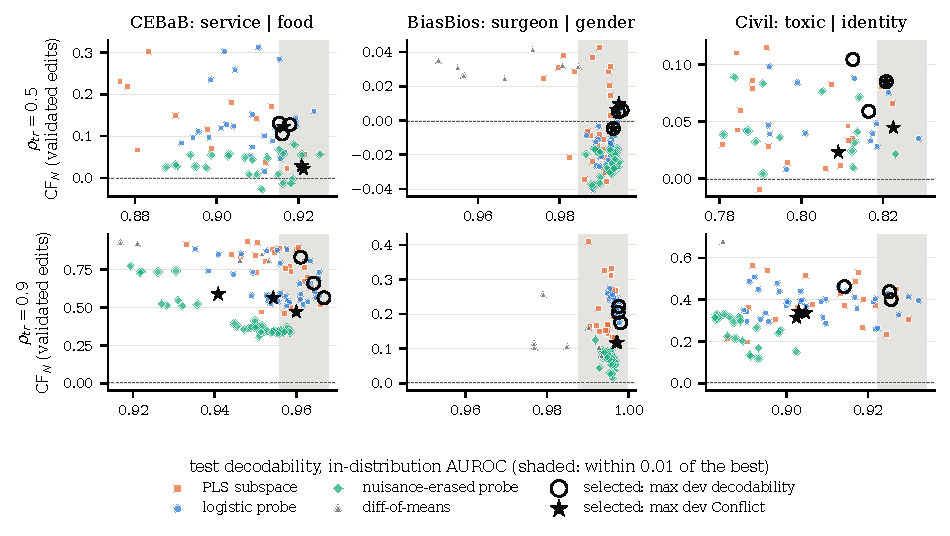
\includegraphics[width=\textwidth]{figs/fig_main_qwen7b.pdf}
\caption{Competitive extractors (\dec{} within 0.05 of the best; Qwen2.5-7B; mean over 3 training samples): test decodability vs.\ nuisance sensitivity $\cfn$ on accepted edits (0: no net shift; 1: the nuisance edit shifts the score as much as a change of target class). Black symbols: the extractor that each training sample selects on development data by maximal \dec{} (ring) or maximal \conf{} (star), standard extractors only. Gemma-2-9B: Appendix~\ref{app:more}.}
\label{fig:main}
\end{figure*}

\begin{table}[t]
\centering\small\setlength{\tabcolsep}{2pt}
\resizebox{\columnwidth}{!}{\begin{tabular}{@{}llccccc@{}}
\toprule
 & & best & \#near & $\cfn$ near-best & $\cfn$ equiv. & \conf{} \\
 & & \dec{} & (equiv.) & range & range & range \\
\midrule
\multicolumn{7}{@{}l}{\emph{$\rhot=0.9$ (correlated training data)}}\\
CEBaB & Q & .966 & 37 (9) & .46--.89 & .54--.81 & .44--.69 \\
 & G & .979 & 39 (8) & .26--.72 & .25--.63 & .57--.82 \\
BiasBios & Q & .998 & 66 (66) & .08--.41 & .08--.41 & .83--.97 \\
 & G & .998 & 66 (63) & .08--.29 & .09--.29 & .92--.97 \\
Civil & Q & .932 & 8 (4) & .24--.45 & .28--.37 & .35--.41 \\
 & G & .940 & 12 (1) & .30--.50 & .35 & .29--.43 \\
\midrule
\multicolumn{7}{@{}l}{\emph{$\rhot=0.5$ (decorrelated)}}\\
CEBaB & Q & .924 & 10 (1) & .02--.28 & .09 & .84--.90 \\
 & G & .960 & 11 (2) & $-$.10--.08 & .01--.02 & .93--.95 \\
BiasBios & Q & .995 & 58 (54) & $-$.04--.04 & $-$.03--.05 & .98--.99 \\
 & G & .995 & 60 (55) & $-$.07--.03 & $-$.06--.03 & .98--.99 \\
Civil & Q & .829 & 4 (2) & .04--.08 & $-$.00--.03 & .81--.83 \\
 & G & .839 & 5 (2) & $-$.02--.07 & $-$.03--$-$.02 & .83--.84 \\
\bottomrule
\end{tabular}
}
\caption{Standard extractors that are near-best (test \dec{} within 0.01 of the best) and, in parentheses, statistically \emph{equivalent} to the best (TOST, margin 0.01). Q: Qwen2.5-7B; G: Gemma-2-9B. $\rhot=0.7$: Appendix~\ref{app:more}.}
\label{tab:near}
\end{table}

\paragraph{Accuracy-matched extractors differ in nuisance sensitivity.} With correlated training data ($\rhot=0.9$), extractors equivalent to the best in decodability span $\cfn$ from \eqCFmincebabQNine{} to \eqCFmaxcebabQNine{} on CEBaB (Qwen; Gemma \eqCFmincebabGNine--\eqCFmaxcebabGNine): for some, rewriting only the food sentence of a review shifts the ``service'' score most of the way to the other service class. On BiasBios \dec{} is at ceiling for nearly all extractors (\eqNbiosQNine{} equivalent to the best), while pronoun swaps shift the occupation score by \eqCFminbiosQNine--\eqCFmaxbiosQNine{} of the surgeon--nurse gap. On Civil few extractors pass the strict equivalence test, but every near-best one has $\conf{}<0.5$: the most decodable toxicity scores rank non-toxic comments about Muslims or LGBTQ people above toxic comments that mention neither. All $\cfn$ values use accepted edits; extractor rankings agree with those on all edits ($\geq$\robAllValMin) and under SD normalization ($\geq$\robSDMin), and signed and absolute $\cfn$ agree at $\rhot\geq0.7$ ($\geq$\robAbsMinSevenUp; Appendix~\ref{app:edits}). Placebo edits barely move scores (median $|\cfn|$ \placeboMin--\placeboMax, vs.\ \nuisAbsNineMin--\nuisAbsNineMax{} for nuisance edits at $\rhot=0.9$).

\paragraph{With decorrelated training, the directional effect mostly disappears.} At $\rhot=0.5$, near-best extractors show little net nuisance shift on BiasBios and Civil (signed $\cfn$ within $\pm0.08$ on accepted edits) and less on CEBaB (\nbCFmincebabQFive--\nbCFmaxcebabQFive, Qwen). Example-level shifts remain on CEBaB, though: median $|\cfn|$ is \absCFcebabQFive{} against a signed \sgnCFcebabQFive{} (Qwen; placebo \placebocebabQFive, for smaller edits). Training-set correlation drives the systematic reliance on the nuisance. A second source is geometric: on CEBaB the target direction and the within-class food direction are highly aligned (cosine \cosMincebab--\cosMaxcebab{} across layers and models; BiasBios \cosMinbios--\cosMaxbios), and this observational geometry alone approximately predicts the counterfactual food sensitivity of the difference-of-means direction trained on decorrelated data (predicted \predMincebab--\predMaxcebab, observed \obsMincebab--\obsMaxcebab; mean absolute error \geomMAEcebab; BiasBios \geomMAEbios). Discriminative probes are much less affected. In a synthetic representation, overlap raises $\cfn$ far more than it changes decodability (Appendix~\ref{app:synthetic}).

\paragraph{Decodability is not a reliable proxy, and on CEBaB target edits do not arbitrate.} Among competitive standard extractors at $\rhot=0.9$, the rank correlation between \dec{} and $\cfn$ ranges from \corrCFmin{} to \corrCFmax{} and changes sign across settings (descriptive bootstrap intervals in Appendix~\ref{app:more}). On CEBaB every near-best extractor, in every regime, responds fully to genuine \emph{service} edits ($\cft$ \cfTmin--\cfTmax) while its food sensitivity ranges over \cfNnbMin--\cfNnbMax. Here only nuisance edits separate more from less selective scores.

\paragraph{A fixed-method comparison.} Choosing each family's layer and hyperparameter on development data, the logistic probe and the nuisance-erased probe are equivalent in \dec{} on BiasBios at $\rhot=0.9$ (difference \fpDdbiosQNine, 90\% CI [\fpLobiosQNine, \fpHibiosQNine], Qwen) yet $\cfn$ is \fpCFlrbiosQNine{} vs.\ \fpCFnebiosQNine{} (Gemma: \fpCFlrbiosGNine{} vs.\ \fpCFnebiosGNine). On CEBaB ($\rhot=0.9$) equivalence is not established (CI up to \fpHicebabQNine) while $\cfn$ falls from \fpCFlrcebabQNine{} to \fpCFnecebabQNine{} (Appendix~\ref{app:more}). Erasure lowers but does not remove nuisance sensitivity: linear guarding on training data is not invariance to edits.

\subsection{Selecting for nuisance selectivity}
\label{sec:selection}

\begin{table}[t]
\centering\small\setlength{\tabcolsep}{2pt}
\resizebox{\columnwidth}{!}{\begin{tabular}{@{}llcccc@{}}
\toprule
 & & \multicolumn{3}{c}{standard extractors} & + erased \\
 & & max \dec{} & max \conf{} & min $|$\leak{}$|$ & max \conf{} \\
\midrule
CEBaB & Q & .69 & .54 ($-$.012) & .50 ($-$.013) & .34 ($-$.007) \\
 & G & .41 & .26 ($-$.005) & .27 ($-$.004) & .11 ($-$.004) \\
BiasBios & Q & .20 & .12 ($-$.001) & .08 ($-$.004) & .03 ($-$.002) \\
 & G & .22 & .12 ($-$.002) & .11 ($-$.006) & .02 ($-$.002) \\
Civil & Q & .43 & .33 ($-$.018) & .31 ($-$.001) & .15 ($-$.034) \\
 & G & .31 & .20 ($-$.015) & .30$^\dagger$ ($-$.006) & .11 ($-$.036) \\
\bottomrule
\end{tabular}
}
\caption{Selecting an extractor on development data at $\rhot=0.9$: test $\cfn$ (accepted edits) of the extractor chosen by maximal \dec{} (standard practice), maximal \conf{}, or minimal $|$\leak{}$|$ among extractors within 0.01 of the best development \dec{}; change in test \dec{} in parentheses. Means over 3 training samples; $^\dagger$: $\cfn$ did not fall in every sample. More criteria: Appendix~\ref{app:more}.}
\label{tab:select}
\end{table}

Practitioners choose a layer and hyperparameters by development accuracy. Table~\ref{tab:select} compares this with nuisance-aware criteria that need nuisance labels on development data but no counterfactuals. Among standard extractors, choosing by \conf{} lowers $\cfn$ in every dataset, model and training sample (by \selStdConfCFmin--\selStdConfCFmax) at a mean \dec{} cost of at most \selStdConfDecMeanWorst{} (\selStdConfDecWorst{} in the worst training sample); it lowers $|\cfn|$ as well, so it is not selecting scores that rely on the opposite of the nuisance. The leakage-constrained rule is similarly effective except on Civil with Gemma; a combined \dec{}$-|$\leak{}$|$ rule behaves similarly (Appendix~\ref{app:more}). When the nuisance-erased probe is available, \conf{} and \dec{}$-|$\leak{}$|$ select it in every sample (the leakage-constrained rule in \neShareMinLeak), and with \conf{} $\cfn$ falls by \selFullConfCFmin--\selFullConfCFmax{} at a mean \dec{} cost of at most \selFullConfDecMeanWorst{} (on Civil, where the nuisance is predictive in-distribution). These accuracy costs are modest, not zero.

\section{Discussion}

Our claim is narrower than ``probes are invalid'': in-distribution decodability is not a reliable proxy for selectivity with respect to a named nuisance. Equally decodable scores can carry very different amounts of nuisance, mainly through correlations in the probe's training data and, in CEBaB, overlapping target and nuisance geometry. A claim that a direction \emph{measures} a concept should name plausible nuisances and report discriminant diagnostics and, where possible, nuisance-only edits; on CEBaB, target edits were passed regardless. Low nuisance sensitivity is necessary discriminant evidence about one nuisance, not construct validity \citep{messick1995validity,licht2025measuring}.

\section*{Limitations}

Each dataset has one nuisance; selectivity for unexamined nuisances is unknown. Edits are filtered by two LLM judges rather than validated by humans; the judges agree poorly to moderately, and accepted pairs may be a selective subset (Appendix~\ref{app:edits}); a blinded stratified sample for human annotation will be released with the code. Rule-based edits leave other cues (first names; the topic of religion or sexuality), and accepting only some edits may select easier pairs, although results on all and accepted pairs agree. $\cfn$ is normalized by the class score gap, which is unstable for weak extractors, so we analyze competitive ones; an effect-size normalization (by the within-cell score SD, akin to Cohen's $d$) ranks extractors similarly ($\geq$\robSDMin). Correlated regimes are produced by resampling; they match natural rates for BiasBios and approximately CEBaB, and are a stress test for Civil. Strict equivalence is established for few extractors on CEBaB and Civil. We study linear readouts of mean-pooled (and, as an ablation, last-token) representations of two 7--9B models; nonlinear probes, SAE features and other models are untested. Our measures concern what a score tracks in text, not what the model computes with it.

\section*{Ethics Statement}

Two datasets involve gender and religious or sexual identity. Concept scores used for auditing or monitoring can encode such attributes while passing accuracy checks; our diagnostics complement, and do not replace, fairness evaluation. The gender swap follows the dataset's binary annotation.

\bibliography{refs}

\appendix

\section{Edit validation and robustness}
\label{app:edits}
Table~\ref{tab:judges} reports, per judge and edit kind, how often the judge found the target kept, the nuisance changed, a fluency drop (edited text rated non-fluent while the source was rated fluent; both judges rate many untouched informal texts as non-fluent, so absolute fluency is not used), and a major other meaning change.\IfFileExists{tables/tab_agreement.tex}{ Table~\ref{tab:agree} gives the agreement of the two judges' accept decisions: agreement is low to moderate ($\kappa$ \kappaMin--\kappaMax), mostly because Qwen3-32B is much stricter (it accepts \qwenPlaceboAccMin--\qwenPlaceboAccMax{} of placebo edits, gpt-oss-120b \gptPlaceboAccMin--\gptPlaceboAccMax), often reporting a fluency drop or a changed target for synonym swaps. Requiring both judges is therefore conservative, and acceptance by both is a filter, not verified correctness; rankings on accepted and on all edits agree closely (Table~\ref{tab:robust}). For Civil, Qwen3-32B judges that swapping the named group changes toxicity in about half of the forward swaps, so few identity swaps survive.}{} The judges were never told which text was edited or which attribute was meant to change. A blinded stratified sample of 25 pairs per dataset and edit kind will be released for human annotation.

\begin{table}[h]
\centering\small\setlength{\tabcolsep}{2pt}
\resizebox{\columnwidth}{!}{\begin{tabular}{@{}llrcccccc@{}}
\toprule
data & edit kind & $n$ & judge & $T$ kept & $N$ changed & fluency drop & major other & accepted \\
\midrule
BiasBios & nuisance & 800 & gpt-oss-120b & .95 & .98 & .02 & .02 & .90 \\
BiasBios & nuisance & 1589 & qwen3-32b & .98 & .98 & .23 & .02 & .74 \\
BiasBios & placebo & 400 & gpt-oss-120b & .96 & .00 & .01 & .00 & .98 \\
BiasBios & placebo & 961 & qwen3-32b & .98 & .00 & .42 & .00 & .58 \\
CEBaB & nuisance & 210 & gpt-oss-120b & .93 & .98 & .05 & .22 & .69 \\
CEBaB & nuisance & 210 & qwen3-32b & .62 & .97 & .15 & .32 & .44 \\
CEBaB & placebo & 158 & gpt-oss-120b & 1.00 & .00 & .08 & .00 & .92 \\
CEBaB & placebo & 158 & qwen3-32b & .91 & .01 & .51 & .00 & .46 \\
CEBaB & target & 125 & gpt-oss-120b & .02 & .10 & .03 & .16 & .76 \\
CEBaB & target & 125 & qwen3-32b & .00 & .08 & .10 & .27 & .55 \\
Civil & nuisance & 762 & gpt-oss-120b & 1.00 & .97 & .00 & .62 & .36 \\
Civil & nuisance & 762 & qwen3-32b & .45 & .98 & .13 & .72 & .17 \\
Civil & nuisance rev & 400 & gpt-oss-120b & 1.00 & .98 & .00 & .36 & .62 \\
Civil & nuisance rev & 400 & qwen3-32b & .63 & .99 & .09 & .53 & .34 \\
Civil & placebo & 480 & gpt-oss-120b & 1.00 & .00 & .06 & .00 & .94 \\
Civil & placebo & 480 & qwen3-32b & .88 & .00 & .53 & .00 & .44 \\
Civil & placebo group & 400 & gpt-oss-120b & 1.00 & .90 & .00 & .06 & .94 \\
Civil & placebo group & 400 & qwen3-32b & .80 & .89 & .06 & .19 & .64 \\
\bottomrule
\end{tabular}
}
\caption{LLM-judge verdicts per edit kind.}
\label{tab:judges}
\end{table}

\IfFileExists{tables/tab_agreement.tex}{%
\begin{table}[h]
\centering\small\setlength{\tabcolsep}{3pt}
\resizebox{\columnwidth}{!}{\begin{tabular}{@{}llrcccc@{}}
\toprule
data & edit kind & $n$ & accept (Qwen3) & accept (gpt-oss) & both & $\kappa$ \\
\midrule
CEBaB & nuisance & 210 & .44 & .69 & .41 & .41 \\
CEBaB & placebo & 158 & .46 & .92 & .44 & .07 \\
CEBaB & target & 125 & .55 & .76 & .52 & .42 \\
BiasBios & nuisance & 800 & .76 & .90 & .72 & .30 \\
BiasBios & placebo & 400 & .60 & .98 & .60 & .05 \\
Civil & nuisance & 762 & .17 & .36 & .13 & .31 \\
Civil & nuisance rev & 400 & .34 & .62 & .29 & .29 \\
Civil & placebo & 480 & .44 & .94 & .43 & .07 \\
Civil & placebo group & 400 & .64 & .94 & .62 & .08 \\
\bottomrule
\end{tabular}
}
\caption{Agreement of the two judges' accept decisions on pairs both rated.}
\label{tab:agree}
\end{table}}{}

\paragraph{Robustness of $\cfn$.} Table~\ref{tab:robust} gives rank correlations, across competitive extractors, between $\cfn$ computed on all vs.\ accepted edits; normalized by $\Delta_T$ vs.\ by the pooled within-cell score SD; signed vs.\ absolute; for the two edit directions separately (CEBaB, BiasBios); and for the forward vs.\ reverse Civil swaps. At $\rhot=0.5$ on CEBaB the signed effect is small while the absolute change is not (median $|\cfn|$ \absCFcebabQFive{} vs.\ signed \sgnCFcebabQFive{}, Qwen), which is why the direction-wise rankings agree less there. Placebo edits are smaller than CEBaB's human rewrites, so the placebo floor is not magnitude-matched for CEBaB. \IfFileExists{tables/tab_placebo.tex}{\input{tables/tab_placebo}}{}

\begin{table}[h]
\centering\small\setlength{\tabcolsep}{2pt}
\resizebox{\columnwidth}{!}{\begin{tabular}{@{}lllccccc@{}}
\toprule
data & model & $\rhot$ & all vs.\ accepted & $\Delta_T$ vs.\ SD norm. & signed vs.\ $|\cdot|$ & direction $+$ vs.\ $-$ & Civil fwd vs.\ rev \\
\midrule
BiasBios & G & 0.5 & 1.00 & +.99 & $-$.93 & +.92 & -- \\
BiasBios & G & 0.7 & 1.00 & +.99 & +.94 & +.97 & -- \\
BiasBios & G & 0.9 & 1.00 & +.99 & 1.00 & +.99 & -- \\
BiasBios & Q & 0.5 & +.99 & +.99 & $-$.54 & +.94 & -- \\
BiasBios & Q & 0.7 & 1.00 & +.99 & +.96 & +.98 & -- \\
BiasBios & Q & 0.9 & 1.00 & +.97 & 1.00 & +.99 & -- \\
CEBaB & G & 0.5 & +.77 & 1.00 & +.13 & +.31 & -- \\
CEBaB & G & 0.7 & +.93 & +.99 & +.89 & +.78 & -- \\
CEBaB & G & 0.9 & +.99 & +.97 & +.99 & +.94 & -- \\
CEBaB & Q & 0.5 & +.88 & +.99 & +.59 & +.69 & -- \\
CEBaB & Q & 0.7 & +.98 & +.99 & +.97 & +.94 & -- \\
CEBaB & Q & 0.9 & +.99 & +.87 & +.99 & +.94 & -- \\
Civil & G & 0.5 & +.98 & +.99 & $-$.24 & -- & +.82 \\
Civil & G & 0.7 & +.99 & +.99 & +.95 & -- & +.92 \\
Civil & G & 0.9 & +.98 & +.94 & +.99 & -- & +.76 \\
Civil & Q & 0.5 & +.93 & +.97 & +.42 & -- & +.76 \\
Civil & Q & 0.7 & +.89 & +.97 & +.99 & -- & +.68 \\
Civil & Q & 0.9 & +.92 & +.93 & 1.00 & -- & +.68 \\
\bottomrule
\end{tabular}
}
\caption{Rank correlations between variants of $\cfn$ across competitive extractors (medians of 3 training samples).}
\label{tab:robust}
\end{table}


\section{Further results}
\label{app:more}
\begin{figure*}[t]
\centering
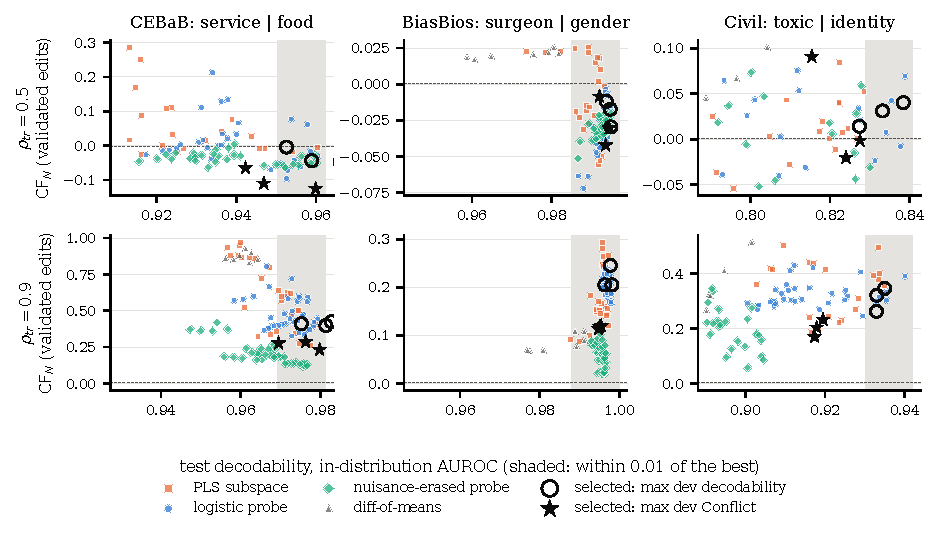
\includegraphics[width=\textwidth]{figs/fig_main_gemma9b.pdf}
\caption{As Figure~\ref{fig:main}, for Gemma-2-9B-it.}
\end{figure*}

\begin{table}[h]
\centering\small\setlength{\tabcolsep}{2pt}
\resizebox{\columnwidth}{!}{\begin{tabular}{@{}llccccc@{}}
\toprule
 & & best & \#near & $\cfn$ near-best & $\cfn$ equiv. & \conf{} \\
 & & \dec{} & (equiv.) & range & range & range \\
\midrule
\multicolumn{7}{@{}l}{\emph{$\rhot=0.7$}}\\
CEBaB & Q & .934 & 18 (0) & .15--.54 & -- & .70--.86 \\
 & G & .967 & 13 (0) & .05--.26 & -- & .86--.93 \\
BiasBios & Q & .995 & 62 (0) & .00--.13 & -- & .96--.99 \\
 & G & .995 & 61 (0) & $-$.01--.10 & -- & .96--.99 \\
Civil & Q & .859 & 5 (0) & .14--.17 & -- & .64--.71 \\
 & G & .869 & 9 (0) & .09--.19 & -- & .66--.69 \\
\bottomrule
\end{tabular}
}
\caption{As Table~\ref{tab:near}, at $\rhot=0.7$ (equivalence tests were run at $\rhot\in\{0.5,0.9\}$ only).}
\end{table}

\begin{table}[h]
\centering\small\setlength{\tabcolsep}{2pt}
\resizebox{\columnwidth}{!}{\begin{tabular}{@{}lllcccc@{}}
\toprule
data & model & $\rhot$ & $\cfn$ & $|\cfn|$ & \conf{} & $|$\leak{}$|$ \\
\midrule
BiasBios & G & 0.5 & $-$.32 [$-$.52, $-$.07] & +.10 [$-$.13, +.33] & +.90 [+.81, +.94] & $-$.24 [$-$.42, $-$.03] \\
BiasBios & G & 0.7 & +.41 [+.23, +.56] & +.40 [+.20, +.55] & +.69 [+.53, +.83] & +.59 [+.44, +.72] \\
BiasBios & G & 0.9 & +.39 [+.13, +.60] & +.39 [+.13, +.61] & +.52 [+.32, +.69] & +.40 [+.13, +.63] \\
BiasBios & Q & 0.5 & $-$.22 [$-$.45, +.05] & $-$.43 [$-$.62, $-$.22] & +.91 [+.84, +.95] & $-$.16 [$-$.38, +.10] \\
BiasBios & Q & 0.7 & $-$.01 [$-$.24, +.22] & $-$.01 [$-$.23, +.23] & +.75 [+.60, +.85] & +.35 [+.15, +.53] \\
BiasBios & Q & 0.9 & +.07 [$-$.24, +.34] & +.07 [$-$.22, +.35] & +.53 [+.32, +.70] & +.32 [+.04, +.53] \\
CEBaB & G & 0.5 & $-$.35 [$-$.57, $-$.03] & $-$.71 [$-$.83, $-$.51] & +.80 [+.64, +.89] & $-$.19 [$-$.46, +.10] \\
CEBaB & G & 0.7 & $-$.43 [$-$.67, $-$.15] & $-$.61 [$-$.77, $-$.36] & +.66 [+.45, +.81] & $-$.29 [$-$.55, +.02] \\
CEBaB & G & 0.9 & $-$.61 [$-$.75, $-$.42] & $-$.65 [$-$.78, $-$.46] & +.68 [+.52, +.78] & $-$.47 [$-$.63, $-$.27] \\
CEBaB & Q & 0.5 & $-$.23 [$-$.49, +.09] & $-$.65 [$-$.82, $-$.40] & +.74 [+.56, +.85] & $-$.08 [$-$.38, +.21] \\
CEBaB & Q & 0.7 & $-$.50 [$-$.67, $-$.23] & $-$.58 [$-$.74, $-$.36] & +.69 [+.51, +.79] & $-$.37 [$-$.57, $-$.11] \\
CEBaB & Q & 0.9 & $-$.43 [$-$.61, $-$.23] & $-$.46 [$-$.63, $-$.27] & +.35 [+.15, +.52] & +.20 [+.01, +.38] \\
Civil & G & 0.5 & +.05 [$-$.32, +.41] & $-$.51 [$-$.69, $-$.26] & +.67 [+.38, +.86] & +.43 [+.10, +.67] \\
Civil & G & 0.7 & $-$.20 [$-$.50, +.15] & $-$.30 [$-$.58, +.02] & +.24 [$-$.07, +.51] & +.53 [+.21, +.82] \\
Civil & G & 0.9 & +.03 [$-$.20, +.26] & $-$.02 [$-$.26, +.22] & $-$.25 [$-$.51, +.05] & +.66 [+.42, +.85] \\
Civil & Q & 0.5 & $-$.09 [$-$.40, +.26] & $-$.42 [$-$.63, $-$.13] & +.70 [+.43, +.84] & +.17 [$-$.22, +.50] \\
Civil & Q & 0.7 & $-$.01 [$-$.36, +.35] & $-$.08 [$-$.38, +.26] & +.24 [$-$.07, +.54] & +.53 [+.17, +.79] \\
Civil & Q & 0.9 & $-$.01 [$-$.29, +.29] & $-$.00 [$-$.30, +.33] & $-$.47 [$-$.69, $-$.20] & +.74 [+.49, +.91] \\
\bottomrule
\end{tabular}
}
\caption{Spearman correlation of test \dec{} with each facet across competitive standard extractors, with 95\% bootstrap CIs over extractors. Hyperparameter variants of one family are not independent, so CIs are descriptive.}
\end{table}

\begin{table}[h]
\centering\small\setlength{\tabcolsep}{2pt}
\resizebox{\columnwidth}{!}{\begin{tabular}{@{}lllcccc@{}}
\toprule
data & model & $\rhot$ & $\Delta$\dec{} [90\% CI] & equiv. & $\cfn$ probe & $\cfn$ erased \\
\midrule
BiasBios & G & 0.5 & $-$.000 [$-$.000, +.000] & yes & $-$.01 & $-$.03 \\
BiasBios & G & 0.9 & +.001 [$-$.001, +.002] & yes & .20 & .06 \\
BiasBios & Q & 0.5 & +.000 [$-$.000, +.000] & yes & $-$.00 & $-$.02 \\
BiasBios & Q & 0.9 & +.001 [+.000, +.002] & yes & .20 & .06 \\
CEBaB & G & 0.5 & +.000 [$-$.000, +.001] & yes & $-$.00 & $-$.01 \\
CEBaB & G & 0.9 & +.004 [$-$.003, +.012] & no & .63 & .14 \\
CEBaB & Q & 0.5 & $-$.003 [$-$.006, +.000] & yes & .13 & .02 \\
CEBaB & Q & 0.9 & +.009 [$-$.003, +.023] & no & .83 & .34 \\
Civil & G & 0.5 & +.008 [+.005, +.011] & no & .01 & $-$.01 \\
Civil & G & 0.9 & +.039 [+.031, +.049] & no & .26 & .18 \\
Civil & Q & 0.5 & +.011 [+.006, +.015] & no & .06 & .04 \\
Civil & Q & 0.9 & +.049 [+.036, +.062] & no & .40 & .28 \\
\bottomrule
\end{tabular}
}
\caption{Logistic probe vs.\ nuisance-erased probe, each family's layer and hyperparameter chosen on development \dec{} (training sample 0). Equiv.: 90\% CI of the \dec{} difference within $\pm0.01$.}
\end{table}

\paragraph{Readout ablation.} Reading the last non-special token instead of mean pooling (Qwen2.5-7B, Table~\ref{tab:pooling}) preserves the pattern: under correlated training, near-best extractors differ substantially in $\cfn$, decorrelated training largely removes it, and Conflict-based selection lowers $\cfn$. On Civil the last-token readout is less decodable and the selection costs considerably more accuracy.

\IfFileExists{tables/tab_pooling.tex}{\begin{table}[h]
\centering\small\setlength{\tabcolsep}{2pt}
\resizebox{\columnwidth}{!}{%
\begin{tabular}{@{}llccccc@{}}
\toprule
 & & \multicolumn{2}{c}{$\rhot=0.9$} & \multicolumn{2}{c}{$\rhot=0.5$} & selection, $\rhot=0.9$ \\
data & readout & best \dec{} & $\cfn$ near-best & best \dec{} & $\cfn$ near-best & $\cfn$: \dec{}$\to$\conf{} ($\Delta$\dec{}) \\
\midrule
CEBaB & mean & .966 & .46--.89 & .924 & .02--.28 & .69$\to$.54 ($-$.012) \\
CEBaB & last token & .968 & .51--.76 & .921 & .15--.27 & .56$\to$.49 ($-$.003) \\
BiasBios & mean & .998 & .08--.41 & .995 & $-$.04--.04 & .20$\to$.12 ($-$.001) \\
BiasBios & last token & .998 & .09--.66 & .994 & $-$.05--.01 & .27$\to$.09 ($-$.005) \\
Civil & mean & .932 & .24--.45 & .829 & .04--.08 & .43$\to$.33 ($-$.018) \\
Civil & last token & .904 & .67--.67 & .794 & .01--.05 & .67$\to$.09 ($-$.156) \\
\bottomrule
\end{tabular}}
\caption{Readout ablation (Qwen2.5-7B, standard extractors, accepted edits): mean pooling vs.\ the last non-special token.}
\label{tab:pooling}
\end{table}
}{}

\begin{table*}[t]
\centering\small
\resizebox{\textwidth}{!}{\begin{tabular}{@{}ll|cccc|ccc@{}}
\toprule
 & & \multicolumn{4}{c|}{standard extractors: $\cfn$ ($\Delta$\dec{})} & \multicolumn{3}{c}{+ erased probe: $\cfn$ ($\Delta$\dec{})} \\
 & & max \dec{} & max \conf{} & min $|$\leak{}$|$ & \dec{}$-|$\leak{}$|$ & max \conf{} & min $|$\leak{}$|$ & \dec{}$-|$\leak{}$|$ \\
\midrule
CEBaB & Q & .69 & .54 ($-$.012) & .50 ($-$.013) & .52 ($-$.008) & .34 ($-$.007) & .34 ($-$.007) & .33 ($-$.011) \\
 & G & .41 & .26 ($-$.005) & .27 ($-$.004) & .26 ($-$.005) & .11 ($-$.004) & .12 ($-$.004) & .14 ($-$.010) \\
BiasBios & Q & .20 & .12 ($-$.001) & .08 ($-$.004) & .10 ($-$.021) & .03 ($-$.002) & .03 ($-$.002) & .03 ($-$.002) \\
 & G & .22 & .12 ($-$.002) & .11 ($-$.006) & .07 ($-$.017) & .02 ($-$.002) & .02 ($-$.001) & .02 ($-$.001) \\
Civil & Q & .43 & .33 ($-$.018) & .31 ($-$.001) & .37 ($-$.041) & .15 ($-$.034) & .31 ($-$.001) & .17 ($-$.038) \\
 & G & .31 & .20 ($-$.015) & .30$^\dagger$ ($-$.006) & .22$^\dagger$ ($-$.020) & .11 ($-$.036) & .30$^\dagger$ ($-$.006) & .11 ($-$.034) \\
\bottomrule
\end{tabular}
}
\caption{All development-set selection criteria at $\rhot=0.9$ (as Table~\ref{tab:select}), for standard extractors and with the nuisance-erased probe.}
\end{table*}


\section{Synthetic representation}
\label{app:synthetic}
We generate $x=T\,u+N\,v+\varepsilon$ in $\mathbb{R}^{256}$ with unit vectors $u,v$ at a chosen cosine (``overlap''), binary $T$ and $N$ with training agreement $\rhot$, and anisotropic Gaussian noise (power-law spectrum). A nuisance edit is exact: $x'=x\pm v$. We fit the same extractors with the same code and compute $\cfn$ on a decorrelated pool. With no overlap, $\cfn$ grows with training correlation (from $\approx0$ at $\rhot=0.5$ to $\approx0.75$ at $0.9$) for every standard extractor: the familiar shortcut. With decorrelated training, $\cfn$ grows with overlap (by \synCFRangeStdMin--\synCFRangeStdMax{} across overlaps for standard extractors) while decodability changes relatively little (by at most \synDecRangeStd; \synDecRangeNe{} for the erased probe; Figure~\ref{fig:synth}). In this low signal-to-noise setting even logistic probes inherit the overlap; in CEBaB, where the target is decoded far better, they inherit much less of it (\S\ref{sec:results}). The synthetic setting illustrates that decodability is largely insensitive to overlap; it is not a model of the real representations.

\begin{figure}[h]
\centering
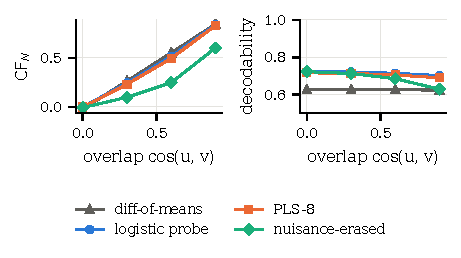
\includegraphics[width=\columnwidth]{figs/fig_synthetic.pdf}
\caption{Synthetic representation, decorrelated training ($\rhot=0.5$): nuisance sensitivity (left) and decodability (right) as target--nuisance overlap grows; means over 5 replicates.}
\label{fig:synth}
\end{figure}


\section{Reproducibility and implementation audit}
\label{app:repro}
All code, data construction, judge outputs and per-extractor metrics will be released; every table and in-text number in this paper is generated from saved results by a script. An automated audit (released) checks that: training, development and test texts are disjoint (CEBaB at the level of review families; two BiasBios test texts and one development text that duplicated training texts were removed); every edit's orientation matches its labels; PLS with $k{=}1$ reproduces the difference of means numerically (cosine 1.000, same orientation); no evaluated text is truncated at 256 tokens on CEBaB and BiasBios, and 0.2\% on Civil; and an independent re-implementation of every metric from the saved raw scores (rank-based AUROC, no shared code) matches the pipeline to $<10^{-8}$. Layers: Qwen hidden states 7, 10, 14, 18, 21, 24, 28 of 28; Gemma 10, 16, 21, 26, 32, 37, 42 of 42. Bootstrap CIs resample review families (CEBaB) or texts within $(T,N)$ cells, and edit pairs.


We do not report residual ``completeness'' \citep{elazar2021amnesic}: whether linear information survives projecting out a subspace is largely fixed by whether the subspace contains the class-mean difference \citep{belrose2023leace}, a property of the estimator rather than of what its score measures.


\end{document}
